\documentclass{report}
\usepackage[portuges]{babel}
\usepackage[utf8]{inputenc}
\usepackage{url}
\usepackage{enumerate}
\usepackage{fancyvrb}
\usepackage{titlesec}
\usepackage{graphicx}
\usepackage{float}
 
%\usepackage{alltt}
%\usepackage{fancyvrb}
\usepackage{listings}
%LISTING - GENERAL
\lstset{
    basicstyle=\small,
    numbers=left,
    numberstyle=\tiny,
    numbersep=5pt,
    breaklines=true,
   frame=tB,
    mathescape=true,
    escapeinside={(*@}{@*)}
}
 
\usepackage{xspace}
 
\parindent=0pt
\parskip=2pt
 
\setlength{\oddsidemargin}{-1cm}
\setlength{\textwidth}{18cm}
\setlength{\headsep}{-1cm}
\setlength{\textheight}{23cm}
 
\def\darius{\textsf{Darius}\xspace}
\def\antlr{\texttt{AnTLR}\xspace}
\def\pe{\emph{Publicação Eletrónica}\xspace}
 
\def\titulo#1{\section{#1}}
\def\super#1{{\em Supervisor: #1}\\ }
\def\area#1{{\em \'{A}rea: #1}\\[0.2cm]}
\def\resumo{\underline{Resumo}:\\ }
 
 
 
\title{Sistemas de Representação de Conhecimento e Raciocínio\\ \textbf{Exercício 3}\\ Relatório de Desenvolvimento}
\author{\textbf{Grupo 18}\\
\\
\\
Cesário Miguel Pereira Perneta - A73883
\\
Luís Miguel Bravo Ferraz - A70824
\\
Rui Pedro Barbosa Rodrigues - A74572
\\
Tiago Miguel Fraga Santos - A74092}
\date{\today}
 
\begin{document}
 
\DefineVerbatimEnvironment{verbatim}{Verbatim}{xleftmargin=.5in}
 
\maketitle
 
\begin{abstract}
Neste relatório será abordada a resolução e verificação do terceiro trabalho prático da unidade curricular de Sistemas de Representação de Conhecimento e Raciocínio.
Será possível encontrar uma detalhada explicação dos predicados elaborados, bem como a apresentaçãao dos scripts utilizados, que visam dar resposta aos requisitos propostos neste trabalho prático.
\end{abstract}
 
\tableofcontents

\chapter{Introdução} \label{intro}

Com a realização deste trabalho o objetivo da equipa docente era a motivação dos alunos para a utilização de sistemas não simbólicos na representação de conhecimento e no desenvolvimento de mecanismos de raciocínio, nomeadamente, Redes Neuronais Artificiais (RNAs) para a resolução de problemas.
Neste terceiro e último exercício pretende-se que seja realizado um estudo que envolva a identificação da qualidade de vinhos (branco e tinto) através do estudo de vários atributos pelos quais, estes são constituidos. 
No próximo capitulo vamos apresentar os \textit{datasets} e fazer uma análise pormenorizada dos mesmos e do problema em questão.


\chapter{Análise do Problema}

De forma a iniciar o trabalho prático os professores disponibilizaram dados que descrevem a qualidade de vinhos através da análise de onze factores. De forma a perceber se uma dada entrada de informação de um vinho tem um selo de qualidade correto face aos seus atributos é preciso fazer uma análise correta dos dados fornecidos, pois são estes que vamos utilizar para efetuar a aprendizagem da rede e respetivos testes. Os ficheiros sao compostos por 11 atributos sendo eles:

\bigbreak
\begin{itemize}
\item{\textbf{fixed acidity} - acidez fixa;} 
\item{\textbf{volatile acidity} - acidez volátil;}
\item{\textbf{citric acid} - acidez citrica;}
\item{\textbf{residual sugar} - açucar residual;}
\item{\textbf{chlorides} - cloretos;}
\item{\textbf{free sulfur dioxide} - dióxido livre de enxofre;}
\item{\textbf{total sulfur dioxide} - dióxido total de enxofre;}
\item{\textbf{density} - densidade;}
\item{\textbf{pH};}
\item{\textbf{sulphates} - sulfatos;}
\item{\textbf{alchohol} - alcool;} 
\end{itemize}
\bigbreak

Os dados dos vinhos foram distribuidos por dois ficheiros, um referente ao vinho tinto (\textit{winequality-red.csv}), e outro ao vinho branco (\textit{winequality-white.csv}).
De forma a procedermos a uma correta análise dos dados e efetuar trabalho sólido e competente, decidimos dividir o trabalho por duas etapas, sendo elas:

\bigbreak
\begin{itemize}
\item{Análise e Tratamento dos Dados para a representação do conhecimento do problema;}
\item{Topologias, aprendizagem e testes das RNA's}
\end{itemize}
\bigbreak

No primeiro ponto, pretendemos fazer uma análise aos dados fornecidos de forma a estabelcer os principais atributos para definir a qualidade dos vinhos, e com o auxilio da ferramenta \textbf{WEKA}, iremos verificar as estatiscas de cada atributo para saber de que forma influenciam a decisão final. Após a analise decidiremos se existe algum atributo a alterar ou se podemos passar para a fase seguinte com os dados inalteráveis.
De seguida, iremos organizar os dados de maneiras diferentes para fornecer a diferentes redes neuronais, com o intuito que no fim possamos avaliar os resultados consoante diferentes neurónios de entrada para diferentes redes. Após conversa com o professor, decidimos que iríamos avançar com três opções.
A primeira opção irá ser composta por duas redes neuronais com 11 neuronios cada uma. Cada neurónio é caracterizado pelos 11 atributos da lista em cima.
A segunda opção pretendemos criar uma redes neuronal com 12 neurónios de entrada. Alem dos atributos já apresentados, o decimo segundo neurónio é caracterizado por um novo atributo:
\bigbreak
\begin{itemize}
\item{\textbf{type} - tipo do vinho(0 - Tinto; 1- Branco);} 
\end{itemize}
\bigbreak

A terceira opção é composta por uma rede neuronal com 22 neuronios de entrada. Cada neurónio é caracterizado pelos seguintes atributos:
\bigbreak
\begin{itemize}
\item{\textbf{fixed\_acidity\_red} - acidez fixa tinta;} 
\item{\textbf{volatile\_acidity\_red} - acidez volátil tinta;}
\item{\textbf{citric\_acid\_red} - acidez citrica tinta;}
\item{\textbf{residual\_sugar\_red} - açucar residual tinta;}
\item{\textbf{chlorides\_red} - cloretos tinta;}
\item{\textbf{free\_sulfur\_dioxide\_red} - dióxido livre de enxofre tinta;}
\item{\textbf{total\_sulfur\_dioxide\_red} - dióxido total de enxofre tinta;}
\item{\textbf{density\_red} - densidade tinta;}
\item{\textbf{pH\_red}; - pH tinto;}
\item{\textbf{sulphates\_red} - sulfatos tinto;}
\item{\textbf{alchohol\_red} - alcool tinto;} 
\item{\textbf{fixed\_acidity\_white} - acidez fixa branco;} 
\item{\textbf{volatile\_acidity\_white} - acidez volátil branco;}
\item{\textbf{citric\_acid\_white} - acidez citrica branco;}
\item{\textbf{residual\_sugar\_white} - açucar residual branco;}
\item{\textbf{chlorides\_white} - cloretos branco;}
\item{\textbf{free\_sulfur\_dioxide\_white} - dióxido livre de enxofre branco;}
\item{\textbf{total\_sulfur\_dioxide\_white} - dióxido total de enxofre branco;}
\item{\textbf{density\_white} - densidade branco;}
\item{\textbf{pH\_white}; - pH branco;}
\item{\textbf{sulphates\_white} - sulfatos branco;}
\item{\textbf{alchohol\_white} - alcool branco;} 
\end{itemize}
\bigbreak

De forma a conseguir, estes dois ultimos \textit{Datasets} tivemos de juntar os dois \textit{datasets} fornecidos pelo prof, e fazer as respetivas alterações como acabaram de ser descritas, quer seja ao nivel de classeificar o vinho conforme o seu tipo ou alterar o nome dos atributos como neste ultimo caso.

Por fim, no terceiro ponto descrito em cima, após ter definido todos os neuronios de entrada para cada uma das redes neuronais, iremos criar cada uma das redes, designando para cada uma a sua topologia, as suas formas de aprendizagem bem como os respetivos testes com o intuito de exercitar as redes e tirar conclusões sobre os resultados obtidos.


















\chapter{Análise e Tratamento dos Dados para a representação do conhecimento do problema}

Neste primeiro capitulo, vamos fazer a análise dos atributos mais importantes com o intuito de perceber quais deles é que influenciam a aprendizagem das redes neuronais em maior escala. 
Para o fazer, utilizamos a ferramentaa \textbf{WEKA} e alguns comandos interpretados pelo \textbf{RStudio} que iremos apresentar em cada secção dos \textit{Datasets}.
Antes da análise detalhada, referimos que em todas as seleções no software \textit{WEKA}, utilizamos o \textit{atributte evaluator} \textbf{CfsSubsetEval} e para o \textit{search method} utilizamos o \textbf{BestFirst}, isto porque, foram os unicos parametros que nos forneceram informações relativas sobre os atributos principais para cada \textit{DataSet}. 
De notar que o \textit{WEKA} oferece muitos mais \textit{attribute evaluators} e \textit{search methods}. A grande maioria não podiam ser utilizados com os nossos dados. O \textit{search method BestFirst} e o \textit{GreedyStepwise} devolviam sempre a mesma seleção de atributos, no entanto, o \textit{GreedyStepwise} não oferece informação sobre os nodos. O \textit{attribute evaluator WrapperSubsetEval} não fazia seleção de qualquer atributo. Utilizando o \textit{search method Ranker} com qualquer um dos possíveis \textit{attribute evaluators} em vez de obtermos uma seleçãoo de atributos tal como os \textit{search methods BestFirst e GreedyStepwise}, obtemos uma classificação de todos os atributos.
Os comandos na linguagem \textbf{R} preocessados no \textit{RStudio} foram os seguintes:
\begin{verbatim}
# --------------
#	For Red and White Wines DataSet
# --------------
# Formula to calculate quality of the wines 
  formula_A <- quality ~ 
  	fixed_acidity + volatile_acidity + 
  	citric_acid + residual_sugar + 
  	chlorides + free_sulfur_dioxide + 
  	total_sulfur_dioxide + density + pH + sulphates + alcohol
 
 # See the most important atributes
  selecao_A <- regsubsets(formula_A,data,method="backward")
  summary(selecao_A)


# --------------
#	For Dataset with 12 atributes
# --------------

 # Formula to calculate quality of the wines
  formula_A <- quality ~ 
  	fixed_acidity + volatile_acidity + 
  	citric_acid + residual_sugar + chlorides + 
  	free_sulfur_dioxide + total_sulfur_dioxide + 
  	density + pH + sulphates + alcohol + type
 
 # See the most important atributes
  selecao_A <- regsubsets(formula_A,data,method="backward")
  summary(selecao_A)


# --------------
#	For Dataset with 22 atributes
# --------------

 # Formula to calculate Quality
  formula_A <- quality ~ 
  fixed_acidity_red + volatile_acidity_red + 
  citric_acid_red + residual_sugar_red + chlorides_red +
  free_sulfur_dioxide_red + total_sulfur_dioxide_red + 
  density_red + pH_red + sulphates_red + alcohol_red + 
  fixed_acidity_white + volatile_acidity_white + 
  citric_acid_white + residual_sugar_white + 
  chlorides_white + free_sulfur_dioxide_white + 
  total_sulfur_dioxide_white + density_white + 
  pH_white + sulphates_white + alcohol_white 
 
 # See the most important atributes
  selecao_A <- regsubsets(formula_A,data,method="backward")
  summary(selecao_A)
\end{verbatim}


Com o auxilio da função \textit{regsubsets} a funcionar através do metodo \textit{backward} conseguimos visualizar com a função \textit{summary} a avaliação dos atributos mais importantes para os quatro \textit{DataSets} que avaliamos.


















\section{DataSet - Vinho Tinto}
\subsection{Script - WEKA}
\begin{verbatim}
=== Run information ===

Evaluator:    weka.attributeSelection.CfsSubsetEval -P 1 -E 1
Search:       weka.attributeSelection.BestFirst -D 1 -N 5
Relation:     winequality-red
Instances:    1599
Attributes:   12
              fixed_acidity
              volatile_acidity
              citric_acid
              residual_sugar
              chlorides
              free_sulfur_dioxide
              total_sulfur_dioxide
              density
              pH
              sulphates
              alcohol
              quality
Evaluation mode:    evaluate on all training data



=== Attribute Selection on all input data ===

Search Method:
	Best first.
	Start set: no attributes
	Search direction: forward
	Stale search after 5 node expansions
	Total number of subsets evaluated: 62
	Merit of best subset found:    0.548

Attribute Subset Evaluator (supervised, Class (numeric): 12 quality):
	CFS Subset Evaluator
	Including locally predictive attributes

Selected attributes: 2,3,10,11 : 4
                     volatile_acidity
                     citric_acid
                     sulphates
                     alcohol
\end{verbatim}

No primeiro \textit{DataSet} analisado, que contem as informações sobre o vinho tinto, como podemos ver em cima, através da análise do script fornecido pelo \textit{WEKA}, os principais atributos que irão ser utilizados nas formulas para aprendizagem das redes neuronais sao: o \textbf{volatile\_acidity}, o \textbf{citric\_acid}, o \textbf{sulphates} e o \textbf{alcohol}.

\subsection{Script - R}
\begin{verbatim}
Subset selection object
Call: regsubsets.formula(formula_Red, data_red, method = "backward")
11 Variables  (and intercept)
                     Forced in Forced out
fixed_acidity            FALSE      FALSE
volatile_acidity         FALSE      FALSE
citric_acid              FALSE      FALSE
residual_sugar           FALSE      FALSE
chlorides                FALSE      FALSE
free_sulfur_dioxide      FALSE      FALSE
total_sulfur_dioxide     FALSE      FALSE
density                  FALSE      FALSE
pH                       FALSE      FALSE
sulphates                FALSE      FALSE
alcohol                  FALSE      FALSE
1 subsets of each size up to 8
Selection Algorithm: backward
         fixed_acidity volatile_acidity citric_acid residual_sugar chlorides free_sulfur_dioxide
1  ( 1 ) " "           " "              " "         " "            " "       " "                
2  ( 1 ) " "           "*"              " "         " "            " "       " "                
3  ( 1 ) " "           "*"              " "         " "            " "       " "                
4  ( 1 ) " "           "*"              " "         " "            " "       " "                
5  ( 1 ) " "           "*"              " "         " "            "*"       " "                
6  ( 1 ) " "           "*"              " "         " "            "*"       " "                
7  ( 1 ) " "           "*"              " "         " "            "*"       "*"                
8  ( 1 ) " "           "*"              "*"         " "            "*"       "*"                
         total_sulfur_dioxide density pH  sulphates alcohol
1  ( 1 ) " "                  " "     " " " "       "*"    
2  ( 1 ) " "                  " "     " " " "       "*"    
3  ( 1 ) " "                  " "     " " "*"       "*"    
4  ( 1 ) "*"                  " "     " " "*"       "*"    
5  ( 1 ) "*"                  " "     " " "*"       "*"    
6  ( 1 ) "*"                  " "     "*" "*"       "*"    
7  ( 1 ) "*"                  " "     "*" "*"       "*"    
8  ( 1 ) "*"                  " "     "*" "*"       "*"  
\end{verbatim}

O scrip fornecido pelo \textit{RStudio} vem confirmar os atributos fornecidos em cima pelo \textit{WEKA} com a exceção que atribui mais influencia ao atributo \textbf{chlorides} em vez do \textbf{citric\_acid}.

Em suma, de forma a carregar os dados de aprendizagem para a rede neuronal que os irá processar, vamos testar as duas versões com duas formulas distintas, uma com os atributos fornecidos pelo \textit{WEKA} e a outra com estes ultimos atributos. 




















\section{DataSet - Vinho Branco}
\subsection{Script - WEKA}
\begin{verbatim}
=== Run information ===

Evaluator:    weka.attributeSelection.CfsSubsetEval -P 1 -E 1
Search:       weka.attributeSelection.BestFirst -D 1 -N 5
Relation:     winequality-white
Instances:    4898
Attributes:   12
              fixed_acidity
              volatile_acidity
              citric_acid
              residual_sugar
              chlorides
              free_sulfur_dioxide
              total_sulfur_dioxide
              density
              pH
              sulphates
              alcohol
              quality
Evaluation mode:    evaluate on all training data



=== Attribute Selection on all input data ===

Search Method:
	Best first.
	Start set: no attributes
	Search direction: forward
	Stale search after 5 node expansions
	Total number of subsets evaluated: 70
	Merit of best subset found:    0.452

Attribute Subset Evaluator (supervised, Class (numeric): 12 quality):
	CFS Subset Evaluator
	Including locally predictive attributes

Selected attributes: 2,5,9,10,11 : 5
                     volatile_acidity
                     chlorides
                     pH
                     sulphates
                     alcohol

\end{verbatim}

No \textit{DataSet} analisado, que contem as informações sobre o vinho branco, como podemos ver em cima, através da análise do script fornecido pelo \textit{WEKA}, os principais atributos que irão ser utilizados nas formulas para aprendizagem das redes neuronais sao: o \textbf{volatile\_acidity}, o \textbf{chlorides}, o \textbf{pH},o \textbf{sulphates} e o \textbf{alcohol}.

\subsection{Script - R}
\begin{verbatim}
Subset selection object
Call: regsubsets.formula(formula_A, data, method = "backward")
11 Variables  (and intercept)
                     Forced in Forced out
fixed_acidity            FALSE      FALSE
volatile_acidity         FALSE      FALSE
citric_acid              FALSE      FALSE
residual_sugar           FALSE      FALSE
chlorides                FALSE      FALSE
free_sulfur_dioxide      FALSE      FALSE
total_sulfur_dioxide     FALSE      FALSE
density                  FALSE      FALSE
pH                       FALSE      FALSE
sulphates                FALSE      FALSE
alcohol                  FALSE      FALSE
1 subsets of each size up to 8
Selection Algorithm: backward
         fixed_acidity volatile_acidity citric_acid residual_sugar chlorides free_sulfur_dioxide
1  ( 1 ) " "           " "              " "         " "            " "       " "                
2  ( 1 ) " "           "*"              " "         " "            " "       " "                
3  ( 1 ) " "           "*"              " "         "*"            " "       " "                
4  ( 1 ) " "           "*"              " "         "*"            " "       " "                
5  ( 1 ) " "           "*"              " "         "*"            " "       " "                
6  ( 1 ) " "           "*"              " "         "*"            " "       " "                
7  ( 1 ) " "           "*"              " "         "*"            " "       "*"                
8  ( 1 ) "*"           "*"              " "         "*"            " "       "*"                
         total_sulfur_dioxide density pH  sulphates alcohol
1  ( 1 ) " "                  " "     " " " "       "*"    
2  ( 1 ) " "                  " "     " " " "       "*"    
3  ( 1 ) " "                  " "     " " " "       "*"    
4  ( 1 ) " "                  "*"     " " " "       "*"    
5  ( 1 ) " "                  "*"     "*" " "       "*"    
6  ( 1 ) " "                  "*"     "*" "*"       "*"    
7  ( 1 ) " "                  "*"     "*" "*"       "*"    
8  ( 1 ) " "                  "*"     "*" "*"       "*"  
\end{verbatim}

O scrip fornecido pelo \textit{RStudio} vem confirmar os atributos fornecidos em cima pelo \textit{WEKA} com a exceção que atribui mais influencia aos atributos \textbf{residual\_sugar} e \textbf{density} em vez do \textbf{chlorides} e do \textbf{sulphates}.

Mais uma vez, de forma a carregar os dados de aprendizagem para a rede neuronal que os irá processar, vamos testar as duas versões com duas formulas distintas, uma com os atributos fornecidos pelo \textit{WEKA} e a outra com estes ultimos atributos.

















\section{DataSet - Vinho Tinto e Branco distinguidos pelo tipo (12 atributos)}
\subsection{Script - WEKA}
\begin{verbatim}
=== Run information ===

Evaluator:    weka.attributeSelection.CfsSubsetEval -P 1 -E 1
Search:       weka.attributeSelection.BestFirst -D 1 -N 5
Relation:     winequality-all-type
Instances:    6497
Attributes:   13
              fixed_acidity
              volatile_acidity
              citric_acid
              residual_sugar
              chlorides
              free_sulfur_dioxide
              total_sulfur_dioxide
              density
              pH
              sulphates
              alcohol
              type
              quality
Evaluation mode:    evaluate on all training data



=== Attribute Selection on all input data ===

Search Method:
	Best first.
	Start set: no attributes
	Search direction: forward
	Stale search after 5 node expansions
	Total number of subsets evaluated: 75
	Merit of best subset found:    0.353

Attribute Subset Evaluator (supervised, Class (numeric): 13 quality):
	CFS Subset Evaluator
	Including locally predictive attributes

Selected attributes: 3,11,12 : 3
                     citric_acid
                     alcohol
                     type
\end{verbatim}

No \textit{DataSet} analisado, que contem as informações sobre o vinho tinto e vinho branco distinguidos por um atributo novo(\textbf{type}), como podemos ver em cima, através da análise do script fornecido pelo \textit{WEKA}, os principais atributos que irão ser utilizados nas formulas para aprendizagem das redes neuronais sao: o \textbf{citric\_acid}, o \textbf{alcohol} e o \textbf{type}.

\subsection{Script - R}
\begin{verbatim}
Subset selection object
Call: regsubsets.formula(formula_A, data, method = "backward")
12 Variables  (and intercept)
                     Forced in Forced out
fixed_acidity            FALSE      FALSE
volatile_acidity         FALSE      FALSE
citric_acid              FALSE      FALSE
residual_sugar           FALSE      FALSE
chlorides                FALSE      FALSE
free_sulfur_dioxide      FALSE      FALSE
total_sulfur_dioxide     FALSE      FALSE
density                  FALSE      FALSE
pH                       FALSE      FALSE
sulphates                FALSE      FALSE
alcohol                  FALSE      FALSE
type                     FALSE      FALSE
1 subsets of each size up to 8
Selection Algorithm: backward
         fixed_acidity volatile_acidity citric_acid residual_sugar chlorides free_sulfur_dioxide
1  ( 1 ) " "           " "              " "         " "            " "       " "                
2  ( 1 ) " "           " "              " "         " "            " "       " "                
3  ( 1 ) " "           " "              " "         " "            " "       " "                
4  ( 1 ) " "           " "              " "         " "            " "       "*"                
5  ( 1 ) " "           " "              " "         " "            " "       "*"                
6  ( 1 ) " "           "*"              " "         " "            " "       "*"                
7  ( 1 ) " "           "*"              " "         " "            "*"       "*"                
8  ( 1 ) " "           "*"              "*"         " "            "*"       "*"                
         total_sulfur_dioxide density pH  sulphates alcohol type
1  ( 1 ) " "                  " "     " " " "       "*"     " " 
2  ( 1 ) " "                  " "     " " " "       "*"     "*" 
3  ( 1 ) "*"                  " "     " " " "       "*"     "*" 
4  ( 1 ) "*"                  " "     " " " "       "*"     "*" 
5  ( 1 ) "*"                  " "     " " "*"       "*"     "*" 
6  ( 1 ) "*"                  " "     " " "*"       "*"     "*" 
7  ( 1 ) "*"                  " "     " " "*"       "*"     "*" 
8  ( 1 ) "*"                  " "     " " "*"       "*"     "*" 
\end{verbatim}

No script do \textit{RStudio}, verificamos que os atributos \textbf{alcohol} e \textbf{type} aparecem em ambos os casos. Neste segundo caso, em vez do protagonismo dado ao \textbf{citric\_acid} é atribuido um papel mais relevante ao \textbf{free\_sulfur\_dioxide} e ao \textbf{sulphates}.

Como nos casos anteriores, de forma a carregar os dados de aprendizagem para a rede neuronal que os irá processar, vamos testar as duas versões com duas formulas distintas, uma com os atributos fornecidos pelo \textit{WEKA} e a outra com estes ultimos atributos.
























\section{DataSet - Vinho Tinto e Branco (22 atributos)}
\subsection{Script - WEKA}
\begin{verbatim}
=== Run information ===

Evaluator:    weka.attributeSelection.CfsSubsetEval -P 1 -E 1
Search:       weka.attributeSelection.BestFirst -D 1 -N 5
Relation:     winequality-all-22
Instances:    6497
Attributes:   23
              fixed_acidity_red
              volatile_acidity_red
              citric_acid_red
              residual_sugar_red
              chlorides_red
              free_sulfur_dioxide_red
              total_sulfur_dioxide_red
              density_red
              pH_red
              sulphates_red
              alcohol_red
              fixed_acidity_white
              volatile_acidity_white
              citric_acid_white
              residual_sugar_white
              chlorides_white
              free_sulfur_dioxide_white
              total_sulfur_dioxide_white
              density_white
              pH_white
              sulphates_white
              alcohol_white
              quality
Evaluation mode:    evaluate on all training data



=== Attribute Selection on all input data ===

Search Method:
	Best first.
	Start set: no attributes
	Search direction: forward
	Stale search after 5 node expansions
	Total number of subsets evaluated: 122
	Merit of best subset found:    0.204

Attribute Subset Evaluator (supervised, Class (numeric): 23 quality):
	CFS Subset Evaluator
	Including locally predictive attributes

Selected attributes: 22 : 1
                     alcohol_white
\end{verbatim}

No \textit{DataSet} analisado, que contem as informações sobre o vinho tinto e vinho branco distinguidos por 22 atributos, como podemos ver em cima, através da análise do script fornecido pelo \textit{WEKA}, só nos é forncedio um atributo que é o \textbf{alcohol\_white}. Desde logo, estranhamos este resultado e decidimos verificar na linguagem \textbf{R} este resultado.


\subsection{Script - R}
\begin{verbatim}
Subset selection object
Call: regsubsets.formula(formula_A, data, method = "backward")
22 Variables  (and intercept)
                           Forced in Forced out
fixed_acidity_red              FALSE      FALSE
volatile_acidity_red           FALSE      FALSE
citric_acid_red                FALSE      FALSE
residual_sugar_red             FALSE      FALSE
chlorides_red                  FALSE      FALSE
free_sulfur_dioxide_red        FALSE      FALSE
total_sulfur_dioxide_red       FALSE      FALSE
density_red                    FALSE      FALSE
pH_red                         FALSE      FALSE
sulphates_red                  FALSE      FALSE
alcohol_red                    FALSE      FALSE
fixed_acidity_white            FALSE      FALSE
volatile_acidity_white         FALSE      FALSE
citric_acid_white              FALSE      FALSE
residual_sugar_white           FALSE      FALSE
chlorides_white                FALSE      FALSE
free_sulfur_dioxide_white      FALSE      FALSE
total_sulfur_dioxide_white     FALSE      FALSE
density_white                  FALSE      FALSE
pH_white                       FALSE      FALSE
sulphates_white                FALSE      FALSE
alcohol_white                  FALSE      FALSE
1 subsets of each size up to 8
Selection Algorithm: backward
         fixed_acidity_red volatile_acidity_red citric_acid_red residual_sugar_red chlorides_red
1  ( 1 ) " "               " "                  " "             " "                " "          
2  ( 1 ) " "               " "                  " "             " "                " "          
3  ( 1 ) " "               " "                  " "             " "                " "          
4  ( 1 ) " "               " "                  " "             " "                " "          
5  ( 1 ) " "               " "                  " "             " "                " "          
6  ( 1 ) " "               " "                  " "             " "                " "          
7  ( 1 ) " "               " "                  " "             " "                " "          
8  ( 1 ) " "               " "                  " "             " "                " "          
         free_sulfur_dioxide_red total_sulfur_dioxide_red density_red pH_red sulphates_red
1  ( 1 ) " "                     " "                      " "         " "    " "          
2  ( 1 ) " "                     " "                      " "         " "    " "          
3  ( 1 ) " "                     " "                      " "         " "    " "          
4  ( 1 ) " "                     " "                      " "         " "    "*"          
5  ( 1 ) " "                     " "                      " "         " "    "*"          
6  ( 1 ) " "                     " "                      " "         " "    "*"          
7  ( 1 ) " "                     " "                      " "         " "    "*"          
8  ( 1 ) " "                     " "                      " "         " "    "*"          
         alcohol_red fixed_acidity_white volatile_acidity_white citric_acid_white
1  ( 1 ) " "         " "                 " "                    " "              
2  ( 1 ) "*"         " "                 " "                    " "              
3  ( 1 ) "*"         " "                 " "                    " "              
4  ( 1 ) "*"         " "                 " "                    " "              
5  ( 1 ) "*"         " "                 " "                    " "              
6  ( 1 ) "*"         " "                 " "                    " "              
7  ( 1 ) "*"         " "                 " "                    " "              
8  ( 1 ) "*"         " "                 " "                    " "              
         residual_sugar_white chlorides_white free_sulfur_dioxide_white total_sulfur_dioxide_white
1  ( 1 ) " "                  " "             " "                       " "                       
2  ( 1 ) " "                  " "             " "                       " "                       
3  ( 1 ) " "                  " "             "*"                       " "                       
4  ( 1 ) " "                  " "             "*"                       " "                       
5  ( 1 ) "*"                  " "             "*"                       " "                       
6  ( 1 ) "*"                  " "             "*"                       "*"                       
7  ( 1 ) "*"                  " "             "*"                       "*"                       
8  ( 1 ) "*"                  " "             "*"                       "*"                       
         density_white pH_white sulphates_white alcohol_white 
1  ( 1 ) " "           " "      " "             "*"           
2  ( 1 ) " "           " "      " "             "*"            
3  ( 1 ) " "           " "      " "             "*"            
4  ( 1 ) " "           " "      " "             "*"            
5  ( 1 ) " "           " "      " "             "*"            
6  ( 1 ) " "           " "      " "             "*"            
7  ( 1 ) " "           " "      "*"             "*"            
8  ( 1 ) " "           "*"      "*"             "*"            
\end{verbatim}

Neste caso, verificamos que os principais atributos são o: \textbf{sulphates\_red}, o \textbf{alcohol\_red}, o \textbf{free\_sulfur\_dioxide\_white} e o \textbf{alcohol\_white}. Após esta análise, decidimos então, carregar os dados de aprendizagem para a rede neuronal que os irá processar, com uma fórmula composta por estes atributos.














































\chapter{Topologias, aprendizagem e testes das RNA's}

Depois do estudo dos atributos, com as fórmulas criadas, falta-nos agora identificar a topologia de rede mais adequada. Decidimos utilizar o algoritmo construtivo para isto. De seguida encontram-se \textit{scripts} utilizados de forma a obter os resultados de alguns dos muitos testes realizados. O valor do threshold utilizado era sempre o mais baixo possível, de modo a conseguir realizar o treino da rede neuronal. Utilizamos o \textit{root-mean-square deviation} (\textbf{RMSE}) para avaliação da qualidade da rede neuronal. O valor da RMSE apresentado nas tabelas é sempre o mais baixo que obtivemos nos testes, à exceção de \textit{outliers} que foram excluídos, pois nunca conseguíamos replica-los, isto devido à natureza das redes neuronais.

\section{Opção A - 2 RNA's abastecidas com 2 DataSets}
\subsection{Script em R - Vinho Tinto}
\begin{verbatim}
# Load needed packages
library(neuralnet)
library(hydroGOF)
library(arules)
library(leaps)

# Read file to memory
data <- read.csv("~/Desktop/SRCR/Trabalhos/Local/TP3/Dados/winequality-red.csv", header=TRUE, sep=";", dec=".")

# Mix data
#data <- data[sample(nrow(data)), ]

# Training set
training <- data[1:1000,]

# Testing set
test <- data[1001:1599,]



# --------------
#	Teste A	-> Weka atributes	
# --------------

 # Formula to calculate quality of the wines 
  formula_A <- quality ~ fixed_acidity + volatile_acidity + citric_acid + residual_sugar + chlorides + free_sulfur_dioxide + total_sulfur_dioxide + density + pH + sulphates + alcohol
 
 # See the most important atributes
  selecao_A <- regsubsets(formula_A,data,method="backward")
  summary(selecao_A)
  
  # Formula to calculate quality of the wines with weka'a most important atributes
  formula_Weka <- quality ~ volatile_acidity + citric_acid + sulphates + alcohol
  
  # Train neural network to predict Quality of the wines
  rna_Weka <- neuralnet(formula_Weka, training, hidden = c(6,4,2), lifesign = "full", linear.output = TRUE, threshold = 0.1)
  
  # Plot neural network
  plot(rna_Weka, rep = "best")
  
  # Define input and test variables
  test_Weka <- subset(test, select=c("volatile_acidity","citric_acid" , "sulphates" ,"alcohol"))
  
  # Test the neural net with new cases
  rna_Weka.results <- compute(rna_Weka, test_Weka)
  
  # Print the results
  results_Weka <- data.frame(current = test$quality, prediction = rna_Weka.results$net.result)
  
  # Round the results
  results_Weka$prediction <- round(results_Weka$prediction, digits = 0)
  
  # Calculate RMSE
  rmse(c(test$quality), c(results_Weka$prediction))
  
  # Plot RMSE
  plot(results_Weka$current, results_Weka$prediction)



# --------------
#	Teste B	-> With R atributtes
# --------------

  # Formula to calculate quality of the wines with weka'a most important atributes
  formula_R <- quality ~ volatile_acidity + chlorides + sulphates + alcohol
  
  # Train neural network to predict Quality
  rna_R <- neuralnet(formula_R, training, hidden = c(5,3), lifesign = "full", linear.output = TRUE, threshold = 0.01)
  
  # Plot neural network
  plot(rna_R, rep = "best")
  
  # Define input and test variables
  test_R <- subset(test, select = c("volatile_acidity","chlorides","sulphates","alcohol"))
  
  # Test the neural net with new cases
  rna_R.results <- compute(rna_R, test_R)
  
  # Print the results
  results_R <- data.frame(current = test$quality, prediction = rna_R.results$net.result)
  
  # Round the results
  results_R$prediction <- round(results_R$prediction, digits = 0)
  
  # Calculate RMSE
  rmse(c(test$quality), c(results_R$prediction))
  
  # Plot RMSE
  plot(results_R$current, results_R$prediction)
\end{verbatim}

\subsection{Script em R - Vinho Branco}
\begin{verbatim}
# Load needed packages
library(neuralnet)
library(hydroGOF)
library(arules)
library(leaps)
# Read file to memory
data <- read.csv("~/Desktop/SRCR/Trabalhos/Local/TP3/Dados/winequality-white.csv", header=TRUE, sep=";", dec=".")

# Mix data
#data <- data[sample(nrow(data)), ]

# Training set
training <- data[1:3000,]

# Testing set
test <- data[3001:4898,]



# --------------
#	Teste A	-> All the atributes	
# --------------

 # Formula to calculate quality of the wines 
  formula_A <- quality ~ fixed_acidity + volatile_acidity + citric_acid + residual_sugar + chlorides + free_sulfur_dioxide + total_sulfur_dioxide + density + pH + sulphates + alcohol
 
 # See the most important atributes
  selecao_A <- regsubsets(formula_A,data,method="backward")
  summary(selecao_A)
  
  
  # Formula to calculate quality of the wines with weka'a most important atributes
  formula_Weka <- quality ~ volatile_acidity + chlorides + pH + sulphates + alcohol
  
  # Train neural network to predict Quality of the wines
  rna_Weka <- neuralnet(formula_Weka, training, hidden = c(6,4,2), lifesign = "full", linear.output = TRUE, threshold = 0.1)
  
  # Plot neural network
  plot(rna_Weka, rep = "best")
  
  # Define input and test variables
  test_Weka <- subset(test, select=c("volatile_acidity","chlorides" , "pH" , "sulphates" ,"alcohol"))
  
  # Test the neural net with new cases
  rna_Weka.results <- compute(rna_Weka, test_Weka)
  
  # Print the results
  results_Weka <- data.frame(current = test$quality, prediction = rna_Weka.results$net.result)
  
  # Round the results
  results_Weka$prediction <- round(results_Weka$prediction, digits = 0)
  
  # Calculate RMSE
  rmse(c(test$quality), c(results_Weka$prediction))
  
  # Plot RMSE
  plot(results_Weka$current, results_Weka$prediction)


  
  # --------------
  #	Teste B	-> With R atributtes
  # --------------
  
  # Formula to calculate quality of the wines with weka'a most important atributes
  formula_R <- quality ~ volatile_acidity + residual_sugar + density + alcohol
  
  # Train neural network to predict Quality
  rna_R <- neuralnet(formula_R, training, hidden = c(5,3), lifesign = "full", linear.output = TRUE, threshold = 0.01)
  
  # Plot neural network
  plot(rna_R, rep = "best")
  
  # Define input and test variables
  test_R <- subset(test, select = c("volatile_acidity","residual_sugar","density","alcohol"))
  
  # Test the neural net with new cases
  rna_R.results <- compute(rna_R, test_R)
  
  # Print the results
  results_R <- data.frame(current = test$quality, prediction = rna_R.results$net.result)
  
  # Round the results
  results_R$prediction <- round(results_R$prediction, digits = 0)
  
  # Calculate RMSE
  rmse(c(test$quality), c(results_R$prediction))
  
  # Plot RMSE
  plot(results_R$current, results_R$prediction)
\end{verbatim}



\subsection{Conclusões e Resultados Obtidos}

\subsubsection{Previsão da Qualidade do Vinho Tinto}

\begin{figure}[H]
\centering
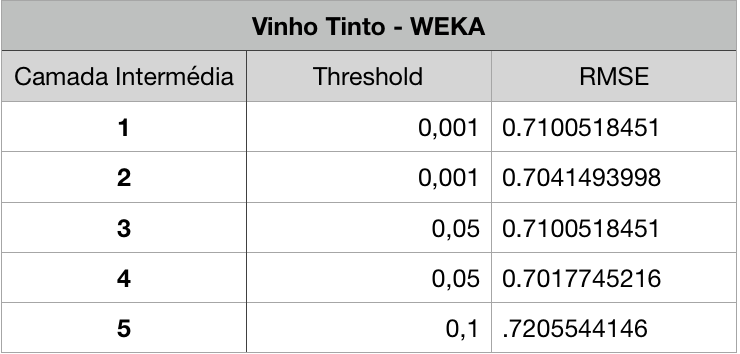
\includegraphics[scale=0.5]{tabelas/1} 
\caption{Valor do RMSE obtido para os dados do weka.}
\end{figure}

\begin{figure}[H]
\centering
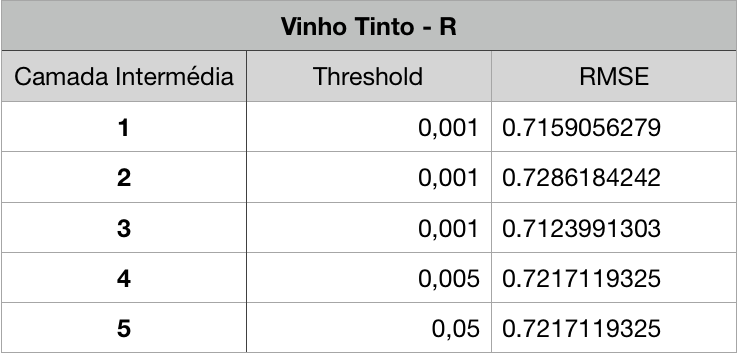
\includegraphics[scale=0.5]{tabelas/2} 
\caption{Valor do RMSE obtido para os dados do R.}
\end{figure} 


Na previsão da qualidade do vinho tinto, através dos dados tratados pelo \textbf{WEKA} o valor mais baixo de \textit{RMSE} face ao valor mais baixo (possivel) de \textit{threshold} é a linha com 4 nodos na camada intermédia, enquanto que nos dados tratados pelo \textit{R} o valor mais baixo de \textit{RMSE} é na camda intermédia com 3 nodos. Embora no segundo caso o \textit{RMSE} seja ligeiramente superior em contrapartida o \textit{threshold} é ligeiramente inferior, deste modo, concluimos que tanto num caso como noutro podemos fazer uma análise correta dos dados.






\subsubsection{Previsão da Qualidade do Vinho Branco}

\begin{figure}[H]
\centering
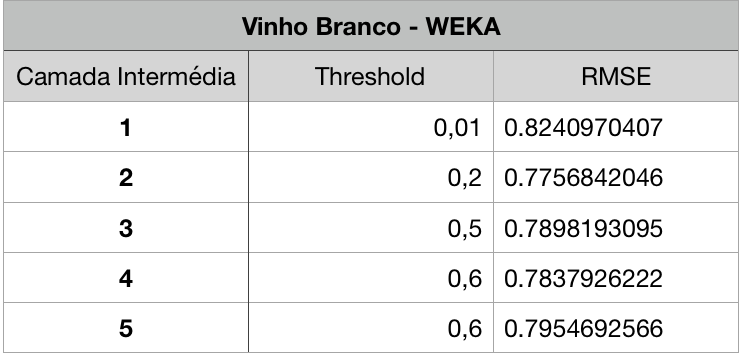
\includegraphics[scale=0.5]{tabelas/3} 
\caption{Valor do RMSE obtido para os dados do weka.}
\end{figure}

\begin{figure}[H]
\centering
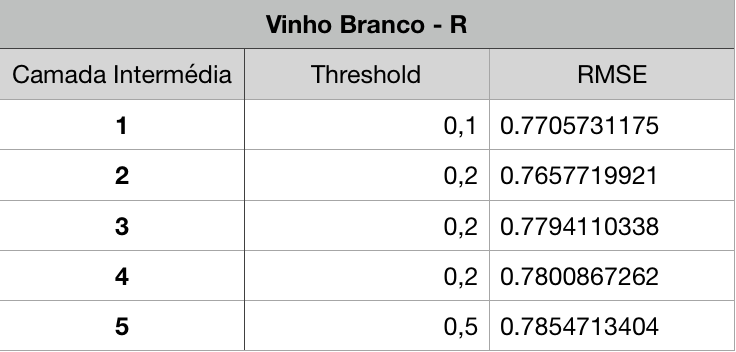
\includegraphics[scale=0.5]{tabelas/4} 
\caption{Valor do RMSE obtido para os dados do R.}
\end{figure} 




Na previsão da qualidade do vinho branco, em ambos os scripts, o valor mais baixo de \textit{RMSE} foi obtido na camada intermédia com dois nodos, sendo o \textit{threshold} igual em ambos os casos. Concluimos que estes valores face aos valores da previsão da qualidade do vinho tinto eram ligeiramente superiores, no entanto, são inferiores aos que vamos ver a seguir.








































\section{Opção B - 1 RNA abastecida por um DataSet de 12 atributos}
\subsection{Script em R}
\begin{verbatim}
# Load needed packages
library(neuralnet)
library(hydroGOF)
library(arules)
library(leaps)

# Read file to memory
data <- read.csv("~/Desktop/SRCR/Trabalhos/Local/TP3/Dados/winequality-all-type.csv", header=TRUE, sep=";", dec=".")

# Mix data
#data <- data[sample(nrow(data)), ]

# Training set
training <- data[1:5000,]

# Testing set
test <- data[5001:6497,]

# --------------
#	Teste A	-> Weka atributes	
# --------------

 # Formula to calculate quality of the wines
  formula_A <- quality ~ fixed_acidity + volatile_acidity + citric_acid + residual_sugar + chlorides + free_sulfur_dioxide + total_sulfur_dioxide + density + pH + sulphates + alcohol + type
 
 # See the most important atributes
  selecao_A <- regsubsets(formula_A,data,method="backward")
  summary(selecao_A)
  
  # Formula to calculate quality of the wines with weka's most important atributes
  formula_Weka <- quality ~ citric_acid + alcohol + type
  
  # Train neural network to predict Quality of the wines
  rna_Weka <- neuralnet(formula_Weka, training, hidden = c(6,4,2), lifesign = "full", linear.output = TRUE, threshold = 0.1)
  
  # Plot neural network
  plot(rna_Weka, rep = "best")
  
  # Define input and test variables
  test_Weka <- subset(test, select=c("citric_acid" , "alcohol" , "type"))
  
  # Test the neural net with new cases
  rna_Weka.results <- compute(rna_Weka, test_Weka)
  
  # Print the results
  results_Weka <- data.frame(current = test$quality, prediction = rna_Weka.results$net.result)
  
  # Round the results
  results_Weka$prediction <- round(results_Weka$prediction, digits = 0)
  
  # Calculate RMSE
  rmse(c(test$quality), c(results_Weka$prediction))
  
  # Plot RMSE
  plot(results_Weka$current, results_Weka$prediction)
  

# --------------
#	Teste B	-> With R atributtes
# --------------

  # Formula to calculate quality of the wines with weka'a most important atributes
  formula_R <- quality ~ free_sulfur_dioxide + sulphates + alcohol + type
  
  # Train neural network to predict Quality
  rna_R <- neuralnet(formula_R, training, hidden = c(5,3), lifesign = "full", linear.output = TRUE, threshold = 0.01)
  
  # Plot neural network
  plot(rna_R, rep = "best")
  
  # Define input and test variables
  test_R <- subset(test, select = c("free_sulfur_dioxide" , "sulphates","alcohol" , "type"))
  
  # Test the neural net with new cases
  rna_R.results <- compute(rna_R, test_R)
  
  # Print the results
  results_R <- data.frame(current = test$quality, prediction = rna_R.results$net.result)
  
  # Round the results
  results_R$prediction <- round(results_R$prediction, digits = 0)
  
  # Calculate RMSE
  rmse(c(test$quality), c(results_R$prediction))
  
  # Plot RMSE
  plot(results_R$current, results_R$prediction)

\end{verbatim}
\bigskip


\subsection{Conclusões e resultados obtidos}

\begin{figure}[H]
\centering
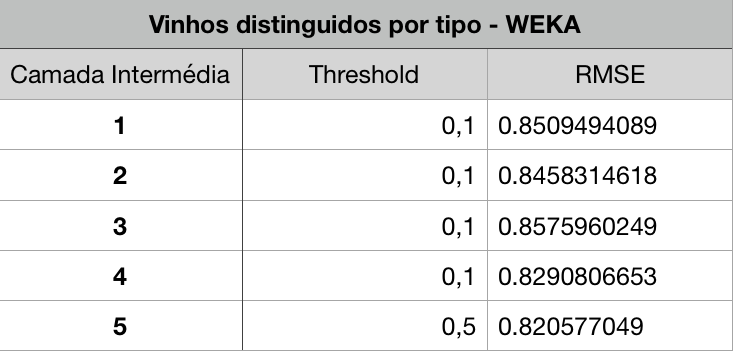
\includegraphics[scale=0.5]{tabelas/5} 
\caption{Valor do RMSE obtido para os dados do weka.}
\end{figure}

\begin{figure}[H]
\centering
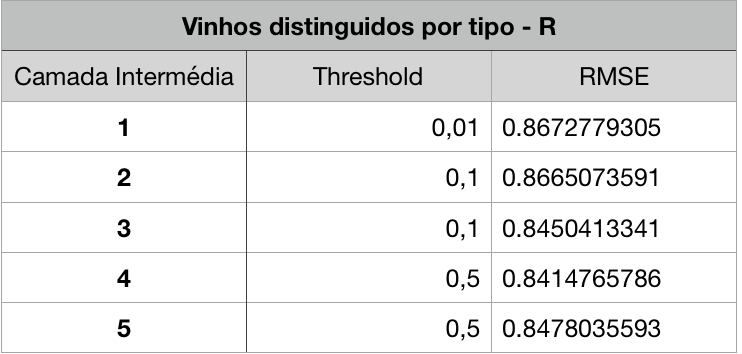
\includegraphics[scale=0.5]{tabelas/6} 
\caption{Valor do RMSE obtido para os dados do R.}
\end{figure} 

\bigskip


Após a observação dos resultados, denotamos de imediato que todos os valores são substancialmente maiores que os anteriores. Embora nao haja muita diferença nos valores do \textit{RMSE} obtidos através do script do \textit{WEKA} e do \textit{R}, para o primeiro caso o valor mais baixo obtido foi na camada intermédia com 5 nodos e um \textit{threshold} de 0,5 enquanto que no segundo caso o valor mais baixo foi alcançado num na camada intermédia com 4 nodos e o mesmo \textit{threshold}.






































\section{Opção C - 1 RNA abastecida por um DataSet de 22 atributos}
\subsection{Script em R}
\begin{verbatim}
# Load needed packages
library(neuralnet)
library(hydroGOF)
library(arules)
library(leaps)

# Read file to memory
data <- read.csv("~/Desktop/SRCR/Trabalhos/Local/TP3/Dados/winequality-all-22.csv", header=TRUE, sep=";", dec=".")

# Mix data
#data <- data[sample(nrow(data)), ]

# Training set
training <- data[1:3000,]

# Testing set
test <- data[3001:4898,]



# --------------
# Teste A -> With R atributtes 
# --------------

 # Formula to calculate Quality
  formula_A <- quality ~ fixed_acidity_red + volatile_acidity_red + citric_acid_red + residual_sugar_red + chlorides_red + free_sulfur_dioxide_red + total_sulfur_dioxide_red + density_red + pH_red + sulphates_red + alcohol_red + fixed_acidity_white + volatile_acidity_white + citric_acid_white + residual_sugar_white + chlorides_white + free_sulfur_dioxide_white + total_sulfur_dioxide_white + density_white + pH_white + sulphates_white + alcohol_white + type
 
 # See the most important atributes
  selecao_A <- regsubsets(formula_A,data,method="backward")
  summary(selecao_A)
  
  # Formula to calculate quality of the wines with weka'a most important atributes
  formula_R <- quality ~ sulphates_red + alcohol_red + free_sulfur_dioxide_white + alcohol_white
  
  # Train neural network to predict Quality
  rna_R <- neuralnet(formula_R, training, hidden = c(5,3), lifesign = "full", linear.output = TRUE, threshold = 0.01)
  
  # Plot neural network
  plot(rna_R, rep = "best")
  
  # Define input and test variables
  test_R <- subset(test, select = c("sulphates_red" , "alcohol_red" , "free_sulfur_dioxide_white" , "alcohol_white"))
  
  # Test the neural net with new cases
  rna_R.results <- compute(rna_R, test_R)
  
  # Print the results
  results_R <- data.frame(current = test$quality, prediction = rna_R.results$net.result)
  
  # Round the results
  results_R$prediction <- round(results_R$prediction, digits = 0)
  
  # Calculate RMSE
  rmse(c(test$quality), c(results_R$prediction))
  
  # Plot RMSE
  plot(results_R$current, results_R$prediction)
\end{verbatim}

\subsection{Conclusões e resultados obtidos}


\begin{figure}[H]
\centering
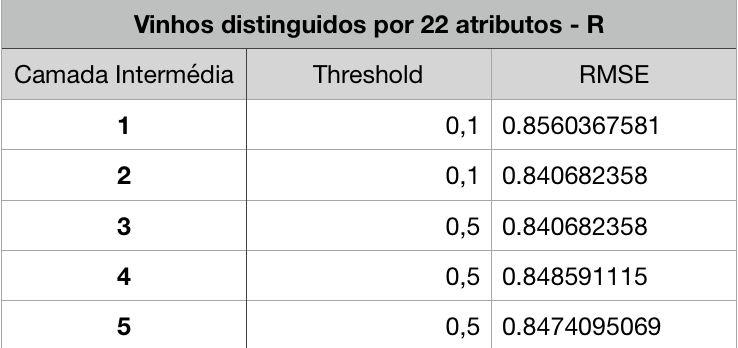
\includegraphics[scale=0.5]{tabelas/7} 
\caption{Valor do RMSE obtido para os dados do R.}
\end{figure} 

\bigskip

Neste último caso o valor mais baixo obtido foi na camada intermédia com 2 nodos e um \textit{threshold} de 0,1. Mais uma vez, em relação ao caso anterior todos os testes que fizemos para esta situação têm no geral um valor do \textit{RMSE} superior que nos oferece o mote para fazermos uma conclusão geral sobre qual a melhor abordagem a usar.




\chapter{Conclusão} \label{concl}

A realização do terceiro exercício desta unidade curricular foi um bom modo de familiarizar com a utilização de sistemas não simbólicos na representação de conhecimento e no desenvolvimento de mecanismos de raciocínio.
A principal dificuldade que encontramos foi exatamente perceber como é que uma rede neuronal funciona. Isto é, como é que as variáveis que colocamos, os número de camadas intermédias e nodos que escolhemos e como é que o \textit{threshold} influenciam o seu treino.
Através da realização de vários testes percebemos que a adição de camadas intermédias pouco influência a qualidade da rede, é a escolha de variáveis e sobretudo, o tratamento dos dados, que mais influenciam a sua qualidade.
Deste modo, através do trabalho realizado, podemos afirmar que a melhor maneira de abordar o problema é através da \textbf{opção A} pois foi com ela que obtemos os melhores valores de \textit{RMSE} com os valores mais baixos de \textit{threshold}.
 
\bibliographystyle{alpha}
\bibliography{relprojLayout}
 
 
\end{document}